% -*- TeX-engine: xetex; eval: (auto-fill-mode 0); eval: (visual-line-mode 1); -*-
% Compile with XeLaTeX

\documentclass[11pt]{article}
%%%%%%%%%%%%%%%%
% Packages
%%%%%%%%%%%%%%%%

\usepackage[top=1cm,bottom=1cm,left=1.5cm,right= 1.5cm]{geometry}
\usepackage[parfill]{parskip}
\usepackage{graphicx, fontspec, xcolor,multicol, enumerate, setspace}
\DeclareGraphicsRule{.tif}{png}{.png}{`convert #1 `dirname #1`/`basename #1 .tif`.png}

%%%%%%%%%%%%%%%%
% No page number
%%%%%%%%%%%%%%%%

\pagestyle{empty}

%%%%%%%%%%%%%%%%
% User defined colors
%%%%%%%%%%%%%%%%

% Pantone 2015 Spring colors
% http://iwork3.us/2014/09/16/pantone-2015-spring-fashion-report/
% update each semester or year

\xdefinecolor{custom_blue}{rgb}{0, 0.70, 0.79} % scuba blue
\xdefinecolor{custom_darkBlue}{rgb}{0.11, 0.31, 0.54} % classic blue
\xdefinecolor{custom_orange}{rgb}{0.97, 0.57, 0.34} % tangerine
\xdefinecolor{custom_green}{rgb}{0.49, 0.81, 0.71} % lucite green
\xdefinecolor{custom_red}{rgb}{0.58, 0.32, 0.32} % marsala

\xdefinecolor{custom_lightGray}{rgb}{0.78, 0.80, 0.80} % glacier gray
\xdefinecolor{custom_darkGray}{rgb}{0.54, 0.52, 0.53} % titanium

%%%%%%%%%%%%%%%%
% Coloring titles, links, etc.
%%%%%%%%%%%%%%%%

\usepackage{titlesec}
\titleformat{\section}
{\color{custom_blue}\normalfont\Large\bfseries}
{\color{custom_blue}\thesection}{1em}{}
\titleformat{\subsection}
{\color{custom_blue}\normalfont}
{\color{custom_blue}\thesubsection}{1em}{}

\newcommand{\ttl}[1]{ \textsc{{\LARGE \textbf{{\color{custom_blue} #1} } }}}

\newcommand{\tl}[1]{ \textsc{{\large \textbf{{\color{custom_blue} #1} } }}}

\usepackage[colorlinks=false,pdfborder={0 0 0},urlcolor= custom_orange,colorlinks=true,linkcolor= custom_orange, citecolor= custom_orange,backref=true]{hyperref}

%%%%%%%%%%%%%%%%
% Instructions box
%%%%%%%%%%%%%%%%

\newcommand{\inst}[1]{
\colorbox{custom_blue!20!white!50}{\parbox{\textwidth}{
	\vskip10pt
	\leftskip10pt \rightskip10pt
	#1
	\vskip10pt
}}
\vskip10pt
}

%%%%%%%%%%%%%%%%
% Timing
%%%%%%%%%%%%%%%%

% 15-20 minutes

%%%%%%%%%%%%%%%%
% Sakai link for course
%%%%%%%%%%%%%%%%

% UPDATE FOR OWN COURSE
% LINK TO ASSIGNMENTS TOOL IN SAKAI

\newcommand{\Sakai}[1]
{\href{https://sakai.duke.edu/portal/site/ba0d1c18-ba55-473f-9d70-b6a1f9559bbe/page/9870858b-a1a9-481e-8497-8a6ffe9e5be2}{Sakai}}

%%%%%%%%%%%
% App Ex number    %
%%%%%%%%%%%

% DON'T FORGET TO UPDATE

\newcommand{\appno}[1]
{4.4}

%%%%%%%%%%%%%%
% Turn on/off solutions       %
%%%%%%%%%%%%%%

% Off
\newcommand{\soln}[1]{
\vskip5pt
}

%% On
%\newcommand{\soln}[1]{
%\textit{\textcolor{custom_darkGray}{#1}}
%}

%%%%%%%%%%%%%%%%
% Document
%%%%%%%%%%%%%%%%

\begin{document}
\fontspec[Ligatures=TeX]{Helvetica Neue Light}

Dr. \c{C}etinkaya-Rundel \hfill Data Analysis and Statistical Inference \\

\ttl{Application exercise \appno{}: \\
ANOVA - Part 1}

\inst{Submit your responses on \Sakai{}, under the appropriate assignment. Only one submission per team is required. One team will be randomly selected and their responses will be discussed.}

\section*{Teacher evaluations}

Many college courses conclude by giving students the opportunity to evaluate the course and the instructor anonymously. In this application exercise we evaluate whether the teaching evaluations for instructors vary by their rank: teaching, tenure track, and tenured. Note that the instructors are evaluated on a 1-5 scale (1-low, 5-high).

The data come from ``Beauty in the classroom: instructors' pulchritude and putative pedagogical productivity'' (Hamermesh and Parker, 2005) found that instructors who are viewed to be better looking receive higher instructional ratings.\footnote{Daniel S. Hamermesh, Amy Parker, Beauty in the classroom: instructors� pulchritude and putative pedagogical productivity, \textit{Economics of Education Review}, Volume 24, Issue 4, August 2005, Pages 369-376, ISSN 0272-7757, 10.1016/j.econedurev.2004.07.013. (\href{http://www.sciencedirect.com/science/article/pii/S0272775704001165}{http://www.sciencedirect.com/science/article/pii/S0272775704001165}).}, which is a dataset we will work with again later in the course.

\begin{center}
\begin{tabular}{l | c | c | c | c | c | c | c | c}
		& Min. & 1st Qu. & Median  &  Mean & 3rd Qu. &   Max. & Std. Dev. & n \\
\hline
teaching	&  3.300 &  3.900  & 4.400&   4.284 &  4.700&   5.000 	& 0.5 & 102 \\
tenure track	& 2.300 &  3.700 &  4.350  & 4.155 &  4.600  & 4.900 & 0.56 & 108 \\
tenured 	&   2.400   & 3.800 &  4.200  & 4.139  & 4.600 &  5.000  & 0.55 & 253
\end{tabular}
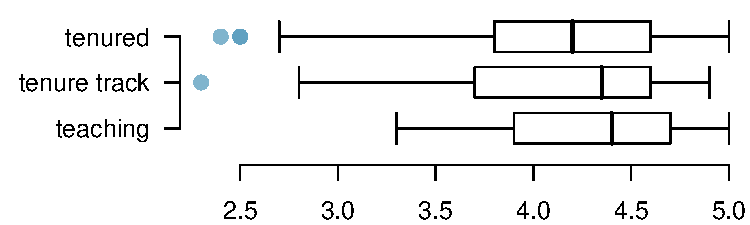
\includegraphics[width=0.6\textwidth]{figures/evals_rank}
\end{center}

%

\begin{enumerate}

\item What is the response and what is the explanatory variable in the ANOVA?

\item State the hypotheses for evaluating whether the average evaluation score varies by rank.

\item Check the conditions for evaluating these hypotheses.

\item Below is a partial ANOVA table. Fill in the blanks. \textit{Hint:} Not all blanks in the table need to be filled, you need to decide which blanks need to be filled.

\begin{center}
\renewcommand{\arraystretch}{1.5}
\begin{tabular}{lrrrrr}
  \hline
 			& Df 		& Sum Sq & Mean Sq 	& F value & Pr($>$F) \\ 
  \hline
evals\$rank 	&  		& 1.59 	&  			& 	 	&  \\ 
  Residuals 	& 	 	& 	 	& 	 		& 		&  \\ 
   \hline
Total			&		& 136.66
\end{tabular}
\end{center}

\item Determine the conclusion of the hypothesis test at $\sigma = 0.10$.

\item Explain what the sum of squares associated with rank (also called $SS_{group}$) and sum of squares associated with the residuals (also called $SS_{error}$) and the total sum of squares mean. You are not being asked to calculate these numbers, only to explain what they mean in context of the data.

\end{enumerate}

%

\end{document}